% Evans second edition, section 3.4.
% English source: printed p. 130; PDF page 147 (1-based).
% Chinese section starts: checked against the chapter-opening list, PDF p. 79.
% Status: editorial study draft with detailed proofs and mathematical notes; no independent review.
\Needspace{65mm}
\section{Introduction to Conservation Laws}
\label{sec:3-4}

\subsection{Shocks and entropy (Evans \S3.4.1)}
We now work in one space dimension:
\[
 u_t+f(u)_x=0,\qquad u(x,0)=g(x).
\]
The conservative form must be retained after smoothness breaks down.
An integral solution is a locally bounded function satisfying
\[
 \int_0^\infty\!\!\int_{\R}[u\phi_t+f(u)\phi_x]\,dx\,dt
       +\int_{\R}g(x)\phi(x,0)\,dx=0
 \tag{CL}
\]
for every smooth compactly supported test function on $\R\times[0,\infty)$.
For smooth $u$, integration by parts proves equivalence with the PDE.
For discontinuous $u$, the expression $f'(u)u_x$ is not an ordinary
product of functions and cannot replace (CL) without additional theory.
\Needspace{45mm}
\PDEAnnotation{先守恒后求导}{光滑时 $f(u)_x=f'(u)u_x$；跳跃时 $u_x$ 含集中测度。守恒形式能直接对 $f(u)$ 作分布求导，避免给不连续函数与 Dirac 的乘积随意赋值。}

\begin{theorem}[Rankine--Hugoniot]\label{thm:3-rh}
Across a smooth shock curve $x=\gamma(t)$ with traces $u_l,u_r$,
an otherwise smooth integral solution must satisfy
\[
 \gamma'(t)(u_r-u_l)=f(u_r)-f(u_l).
 \tag{RH}
\]
For unequal states, the speed is the secant slope of $f$.
\end{theorem}
\begin{expandedproof}
Write locally $u=u_l+(u_r-u_l)\mathbf1_{\{x>\gamma(t)\}}$,
with the smooth extensions on each side understood.
The singular part of $u_t$ is $-\gamma'[u]\delta_{x=\gamma(t)}$;
that of $f(u)_x$ is $[f]\delta_{x=\gamma(t)}$.
Here $[u]=u_r-u_l$ and $[f]=f(u_r)-f(u_l)$.
The regular parts vanish by the PDE on each side.
The remaining distribution is zero precisely when (RH) holds.
Equivalently, integrate each smooth side of (CL) and add their
oppositely oriented interface fluxes.
\end{expandedproof}

For strictly convex $f$, an admissible shock has $u_l>u_r$.
Its speed satisfies
$f'(u_r)<\gamma'<f'(u_l)$, since secant slopes lie strictly between
endpoint tangent slopes.
Characteristics enter the shock from both sides.
An upward jump also satisfies (RH) with its secant speed, but would
send characteristics outward and is rejected by entropy.


\PDEBodyDiagram{3.4}{Shock speed is a secant slope.}
{For $f(u)=u^2/2$, the secant between $u_R=0.2$ and $u_L=1.4$ has slope $\sigma=0.8$. The tangent slopes satisfy $0.2<0.8<1.4$, so characteristics from both sides enter the shock. Reversing the spatial states keeps the secant slope but violates the compression direction.}
{ch03-flux-chord}

\paragraph{Why weak conservation alone is not unique.}
For Burgers flux $f(u)=u^2/2$ and data $g=0$ on $x<0$, $g=1$ on $x>0$,
both the upward step moving at speed $1/2$ and
\[
 u(x,t)=\begin{cases}
 0,&x\leq0,\\ x/t,&0<x<t,\\1,&x\geq t
 \end{cases}
\]
satisfy (CL). In the fan the PDE is
$-x/t^2+(x/t)(1/t)=0$, and both interfaces are continuous.
Each candidate attains the same initial data in local $L^1$.
Only the fan satisfies the one-sided bound derived below.
\Needspace{45mm}
\PDEAnnotation{跳跃条件不负责筛选方向}{Rankine--Hugoniot 只保证接口两侧通量守恒，上跳和下跳都可能满足。熵条件额外保留压缩型跳跃，排除向外散开的非物理解。}

\paragraph{Convex entropy pairs: an editorial explanation.}
For smooth convex $\eta$, define $q$ by $q'=\eta'f'$.
A smooth solution satisfies $\eta(u)_t+q(u)_x=0$.
For the viscous equation $u_t+f(u)_x=\varepsilon u_{xx}$,
\[
 \eta(u)_t+q(u)_x
 =\varepsilon\partial_{xx}\eta(u)
       -\varepsilon\eta''(u)|u_x|^2
 \leq\varepsilon\partial_{xx}\eta(u).
\]
If bounded viscous solutions converge strongly locally, their limit
therefore satisfies the distributional entropy inequality.
This is a conditional explanation of the selection rule, not a proof
of viscous existence or convergence.

For a downward shock $l=u_l>u_r=r$ with secant speed $s$, let
$C(v)=f(v)-f(r)-s(v-r)\leq0$ on $[r,l]$.
The singular entropy coefficient is
\[
 [q]-s[\eta]=-\int_r^l\eta'(v)C'(v)\,dv
            =\int_r^l\eta''(v)C(v)\,dv\leq0.
\]
Thus the convex entropy inequality selects the same direction.
For general nonsmooth solutions this chapter uses the source's
one-sided derivative condition as its explicit uniqueness class.

\subsection{The Lax--Oleinik construction (Evans \S3.4.2)}
\label{sec:3-laxoleinik}
Assume $f$ smooth and $f''\geq\theta>0$ on $\R$, and $g\in L^\infty$.
An additive constant in $f$ does not affect the PDE; take $f(0)=0$.
Let
\[
 P(x)=\int_0^xg(y)\,dy,\qquad
 L=f^*,\qquad G=(f')^{-1}=L'.
\]
The potential
\[
 W(x,t)=\min_y\{tL((x-y)/t)+P(y)\}
 \tag{LOP}
\]
is a Hopf--Lax solution of $W_t+f(W_x)=0$.
The candidate conservation-law solution is $u=W_x$ a.e.
\Needspace{45mm}
\PDEAnnotation{HJ 解是守恒律解的原函数}{$W_t+f(W_x)=0$ 对空间作分布求导，就得到 $u_t+f(u)_x=0$。给初始原函数 $P$ 加常数只会给 $W$ 加同一常数，不改变 $u$ 或最优起点。}
Since $f'$ is strictly increasing and onto, $G$ exists and is
$1/\theta$-Lipschitz. Differentiating the convex dual at its unique
maximizer gives $L'=G$ and $L''=1/f''(G)>0$.

\begin{theorem}[Source Theorem 1]\label{thm:3-lo}
For each $t>0$, minimizing starting points in (LOP) are ordered with $x$.
The minimizer is unique except at at most countably many $x$.
At differentiability points of $W$,
\[
 \boxed{u(x,t)=G((x-y(x,t))/t).}
 \tag{LO}
\]
\end{theorem}
\begin{expandedproof}
\paragraph{1. Ordering and countability.}
Put $c(x,y)=tL((x-y)/t)$.
Its mixed derivative is $c_{xy}=-L''((x-y)/t)/t<0$.
If $x_1<x_2$ and proposed minimizers had $y_1>y_2$,
integration of this mixed derivative on the rectangle gives
\[
 c(x_1,y_2)+c(x_2,y_1)<c(x_1,y_1)+c(x_2,y_2).
\]
Adding $P(y_1)+P(y_2)$ contradicts the sum of the two minimizing
inequalities. Hence every minimizer at $x_1$ is at most every minimizer
at $x_2$.
The minimum sets are nonempty compact sets by coercivity.
If a set has two distinct endpoints $y_-<y_+$, its interval
$(y_-,y_+)$ is disjoint from the corresponding intervals for other $x$.
Assigning a rational point to each nonempty interval proves there are
at most countably many such $x$.

\Needspace{45mm}
\PDEAnnotation{可数例外指固定的时间切片}{每个多重最优点对应一个互不相交的起点开区间，再各选一个有理数，才得到可数性。这不表示整个时空只存在可数个激波点，也不等于全局光滑。}
\paragraph{2. Differentiate the value without differentiating the optimizer.}
For a fixed minimizing $y$, use that same point as a competitor at
$x+h$. Then
$W(x+h,t)-W(x,t)\leq c(x+h,y)-c(x,y)$.
For positive and negative $h$, differentiability of $W$ gives
$W_x=L'((x-y)/t)=G((x-y)/t)$.
This works even if $P$ is not differentiable at the minimizing $y$.
Strict monotonicity of $G$ also forces uniqueness of $y$ at such a point.
\end{expandedproof}
\Needspace{45mm}
\PDEAnnotation{最优起点的跳跃产生激波}{$y(x,t)$ 保持单调，但可发生跳跃。跨过竞争分支时，$(x-y)/t$ 随之下降，因此 $u=G((x-y)/t)$ 出现向下跳跃；这把变分选择和熵方向联系起来。}

\begin{theorem}[Integral solution and initial trace; source Theorem 2]
The construction gives a bounded integral solution of (CL).
It satisfies $u(\cdot,t)\to g$ in $L^1_{\mathrm{loc}}$ as $t\downarrow0$.
\end{theorem}
\begin{expandedproof}
First $W$ is spatially Lipschitz with constant $\|g\|_\infty$, hence
$|u|\leq\|g\|_\infty$ a.e.
The a.e. HJ equation $W_t+f(W_x)=0$ is an equality of locally integrable
functions. Multiply it by $\phi_x$.
Integration by parts first in time and then in space gives
\[
 \iint W_t\phi_x
 =-\iint W\phi_{xt}-\int P\phi_x(\cdot,0)
 =\iint W_x\phi_t+\int g\phi(\cdot,0).
\]
All supports are compact and $W$ is Lipschitz; thus these are valid
weak integration identities. Substituting $u=W_x$ proves (CL).

To strengthen initial recovery, fix a Lebesgue point $x$ of $g$,
with value $g_0$. Then
$P(x+h)=P(x)+g_0h+o(|h|)$.
The coercive minimizer bound gives $|x-y|/t\leq R$ uniformly.
Writing $y=x-tv$, the minimizing objective becomes
\[
 P(x)+t[L(v)-g_0v]+o(t)
\]
uniformly for $|v|\leq R$.
The strictly convex function $L(v)-g_0v$ has unique minimizer
$v_*=f'(g_0)$. Compactness implies every minimizing velocity tends
to $v_*$: otherwise a convergent subsequence away from $v_*$ would
minimize the limiting strictly convex objective.
Formula (LO) therefore gives $u(x,t)\to G(v_*)=g_0$.
The uniform $L^\infty$ bound and dominated convergence on compact
intervals give the asserted local $L^1$ convergence.
\end{expandedproof}

\subsection{A one-sided estimate and uniqueness (Evans \S3.4.3)}
\label{sec:3-entropy}
For the Lax--Oleinik solution, choose a monotone minimizing
representative $y(x,t)$ (for example the largest minimizer).
For $z>0$,
$y(x+z,t)\geq y(x,t)$ and therefore
\[
 u(x+z,t)-u(x,t)\leq \frac{z}{\theta t}.
 \tag{OS}
\]
Indeed the corresponding velocity can increase by at most $z/t$;
$G$ is increasing and $1/\theta$-Lipschitz.
If the velocity decreases, the displayed upper bound is automatic.
Thus $u(x,t)-x/(\theta t)$ is nonincreasing at fixed $t$.
It has one-sided limits and only downward jumps, although its
decrease may be arbitrarily steep.
\Needspace{45mm}
\PDEAnnotation{单边界允许激波}{约束是 $u(x+z)-u(x)\leq Cz/t$，不是绝对值的 Lipschitz 界。向下跳跃完全允许，向上跳跃则被禁止；这正适合包含压缩激波的解空间。}

The source's entropy class consists of bounded integral solutions
with a representative satisfying
$u(x+z,t)-u(x,t)\leq C(1+t^{-1})z$ for $z>0$ a.e.
The term $1$ permits a more general bound than (OS).

\begin{theorem}[Source Theorem 3]
For smooth convex $f$, an entropy solution in this one-sided class
with a prescribed bounded initial datum is unique up to null sets.
Uniform convexity is used for the explicit Lax--Oleinik construction,
but plain convexity suffices for this uniqueness statement.
\end{theorem}
\begin{expandedproof}[dual transport, with two separate small-time scales]
Let $w=u-\widetilde u$ and
\[
 b(x,t)=\int_0^1f'(\lambda u+(1-\lambda)\widetilde u)\,d\lambda .
\]
Then $f(u)-f(\widetilde u)=bw$. Subtracting the two integral identities
with the same initial datum gives
\[
 \iint w(\phi_t+b\phi_x)=0
 \tag{DU}
\]
for tests compactly supported in $\R\times[0,\infty)$.
The common data cancel exactly; no pointwise initial derivative is assumed.

\paragraph{1. Regularize the velocity and control its upper derivative.}
Smooth bounded extensions of $u,\widetilde u$ in space-time by
nonnegative kernels and set
$b_\varepsilon=\int_0^1f'(\lambda u_\varepsilon+
(1-\lambda)\widetilde u_\varepsilon)\,d\lambda$.
The coefficients are uniformly bounded, say $|b_\varepsilon|\leq R$,
and converge a.e. to $b$.
For $t>2\varepsilon$, the one-sided bound, averaged against the kernel
and divided by $z$, gives
$(u_\varepsilon)_x,(\widetilde u_\varepsilon)_x
 \leq C'(1+t^{-1})$.
Because $f''\geq0$ and is bounded on the common bounded value range,
\[
 (b_\varepsilon)_x
 =\int_0^1 f''(\lambda u_\varepsilon+(1-\lambda)\widetilde u_\varepsilon)
       [\lambda(u_\varepsilon)_x+
                    (1-\lambda)(\widetilde u_\varepsilon)_x]\,d\lambda
 \leq C''(1+t^{-1}).
\]
Negative derivatives need no lower bound.

\paragraph{2. Solve a smooth backward test equation.}
Fix $\psi\in C_c^\infty(\R\times(0,T))$.
Let $v_\varepsilon$ solve
$(v_\varepsilon)_t+b_\varepsilon(v_\varepsilon)_x=\psi$ with
$v_\varepsilon(\cdot,T)=0$.
The characteristic formula is
\[
 v_\varepsilon(x,t)
 =-\int_t^T\psi(X_\varepsilon(s;x,t),s)\,ds,\qquad
 \dot X_\varepsilon=b_\varepsilon(X_\varepsilon,s).
\]
Bounded speed makes all its supports lie in a fixed spatial interval.
It vanishes near $T$, so it is an admissible smooth test in (DU).

For any fixed $\delta>0$, $\varepsilon<\delta/2$,
differentiate the flow in $x$:
\[
 \partial_xX_\varepsilon(s;x,t)
 =\exp\left(\int_t^s(b_\varepsilon)_x(X_\varepsilon(\tau),\tau)\,d\tau\right).
\]
The upper derivative bound for $t\geq\delta$ gives a uniform finite
bound on this positive factor.
Differentiating the test formula therefore yields
$|(v_\varepsilon)_x|\leq C_\delta$ for $\delta\leq t\leq T$.

\Needspace{45mm}
\PDEAnnotation{一维保序带来变差守恒}{光滑流关于初始位置严格递增，因此复合流只是重新排列同一条曲线上的取值次序，不增加总变差。这里不需要流的导数在零时刻附近有统一上界。}
\paragraph{3. A fixed early interval controls total variation.}
Choose a fixed $t_*>0$ so that $\psi=0$ for $0<t<2t_*$.
For $t\leq t_*$, $v_\varepsilon$ is transported unchanged along
characteristics to time $t_*$.
A one-dimensional smooth flow preserves order and is a diffeomorphism
of $\R$ (its speed is bounded). Hence composition with this flow
preserves total variation:
\[
 \int_{\R}|(v_\varepsilon)_x(x,t)|\,dx
 =\operatorname{Var}v_\varepsilon(\cdot,t)
 =\operatorname{Var}v_\varepsilon(\cdot,t_*)\leq D.
\]
The final bound follows from the derivative bound at the fixed $t_*$
and the fixed compact support. Crucially, $D$ is independent of both
$\varepsilon$ and a later splitting time $\delta<t_*$.

\paragraph{4. Pass the dual identity to the limit.}
Use $v_\varepsilon$ in (DU):
\[
 \iint w\psi=\iint w(b_\varepsilon-b)(v_\varepsilon)_x.
\]
Split at $t=\delta$, with $0<\delta<t_*$.
On $[\delta,T]$ the integrand tends to zero by dominated convergence,
using $C_\delta$ and common compact support.
On $(0,\delta)$, boundedness of $w,b_\varepsilon,b$ and the
total-variation estimate bound its absolute integral by $C D\delta$.
First let $\varepsilon\downarrow0$ for this fixed $\delta$,
then let $\delta\downarrow0$.
Thus $\iint w\psi=0$ for every interior test $\psi$, so $w=0$ a.e.
\end{expandedproof}
\Needspace{45mm}
\PDEAnnotation{两个小时间不能混用}{先固定源项消失的时段 $t_*$，用它得到统一的变差界；再另取 $\delta<t_*$ 切开误差。若让估计常数也随 $\delta$ 发散，就不能仅凭区间长度趋零断言误差消失。}


\subsection{Riemann's problem (Evans \S3.4.4, Theorem 4)}
For $g=u_l$ on $x<0$ and $g=u_r$ on $x>0$, the entropy solution for
a strictly convex flux is as follows.
If $u_l>u_r$, it is a shock with speed
$s=[f(u_l)-f(u_r)]/(u_l-u_r)$.
If $u_l<u_r$, it is the rarefaction
\[
 u(x,t)=\begin{cases}
 u_l,&x/t\leq f'(u_l),\\
 G(x/t),&f'(u_l)<x/t<f'(u_r),\\
 u_r,&x/t\geq f'(u_r).
 \end{cases}
 \tag{RF}
\]
Equal states give a constant solution.
\begin{expandedproof}
The shock satisfies the PDE off its interface, (RH) on it, and the
downward entropy direction.
In the fan, $u_t=-(x/t^2)G'(x/t)$ and
$f'(u)u_x=(x/t)G'(x/t)/t$, which cancel.
The fan joins continuously to both constant states and
$u_x=G'(x/t)/t\leq1/(\theta t)$.
Both candidates are integral solutions and approach their Riemann data
locally in $L^1$; the transition region has width $O(t)$.
The entropy uniqueness theorem just proved identifies them as the
selected solutions.
\end{expandedproof}
\begin{center}
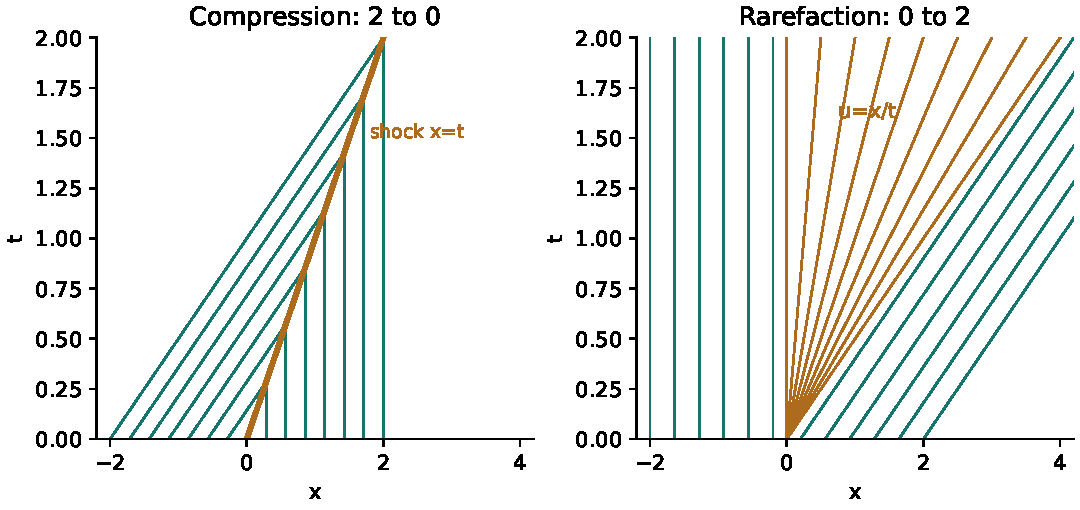
\includegraphics[width=\linewidth]{output/figures/ch03-riemann-characteristics.pdf}
\end{center}
\noindent\textit{Editorial figure.} For Burgers flow, a downward step
compresses characteristics into a shock; an upward step opens a
rarefaction fan. Both geometries use the same flux, but different data.

\subsection{Long-time decay and N-waves (Evans \S3.4.5)}
For this subsection assume $f(0)=0$, $f$ smooth, and
$0<\theta\leq f''\leq\Theta<\infty$.
These convenient sufficient hypotheses ensure uniform convexity of
both $f$ and $L=f^*$, as required in the source asymptotic arguments.
Write $\sigma=f'(0)$ and $d=f''(0)$.

\begin{theorem}[Supremum decay; source Theorem 5]
For bounded integrable initial data,
$\|u(\cdot,t)\|_\infty\leq C t^{-1/2}$.
\end{theorem}
\begin{expandedproof}
The primitive $P$ in (LOP) is bounded by $M=\|g\|_1$.
Duality gives $L(\sigma)=0$, $L'(\sigma)=0$.
Since $L''\geq1/\Theta$,
$L(v)\geq(v-\sigma)^2/(2\Theta)$.
Compare a minimizing $y$ with $y_0=x-\sigma t$:
\[
 \frac{|x-y-\sigma t|^2}{2\Theta t}-M
 \leq tL((x-y)/t)+P(y)\leq P(x-\sigma t)\leq M.
\]
Thus $|(x-y)/t-\sigma|\leq C/\sqrt t$.
As $G(\sigma)=0$ and $G$ is $1/\theta$-Lipschitz,
formula (LO) gives the claim.
\end{expandedproof}
\Needspace{45mm}
\PDEAnnotation{衰减的是高度，不一定是质量}{波的高度可按 $t^{-1/2}$ 降低，同时宽度按 $\sqrt t$ 增长。积分质量不一定趋零，所以长期形状应和一个展开的 N 波比较，而非只和零比较。}

Suppose additionally $\supp g\subset[-R,R]$.
Use the equivalent primitive $P(x)=\int_{-\infty}^xg$,
so $P_-=0$, $P_+=m=\int g$.
Let $P_*=\min P$,
\[
 p=-2P_*,\qquad q=2(m-P_*),\qquad p,q\geq0.
\]
The associated N-wave is
\[
 N(x,t)=\begin{cases}
 (x-\sigma t)/(dt),
   &-\sqrt{pdt}<x-\sigma t<\sqrt{qdt},\\
 0,&\text{otherwise}.
 \end{cases}
 \tag{NW}
\]
Its negative and positive signed areas are $-p/2$ and $q/2$,
so $\int N=(q-p)/2=m$.
\Needspace{45mm}
\PDEAnnotation{N 波参数由原函数最低点决定}{$p,q$ 不是初值正负质量各乘二。例如先取正脉冲再取等质量负脉冲，原函数始终非负且最终回零，此时 $p=q=0$，即使初值两种符号都有。}
\begin{theorem}[Source Theorem 6]
If $p,q>0$, then $\|u(\cdot,t)-N(\cdot,t)\|_1\leq C t^{-1/2}$.
\end{theorem}
\begin{expandedproof}[locating the edges before integrating the error]
Pass to the moving coordinate $\xi=x-\sigma t$ and put
$\ell(v)=L(\sigma+v)$. Then
$\ell(0)=\ell'(0)=0$ and $\ell''(0)=1/d$.
The minimizing velocity bound just proved is $|(\xi-y)/t|\leq C/\sqrt t$.
Taylor expansion on this fixed small-velocity range gives
\[
 t\ell((\xi-y)/t)=\frac{(\xi-y)^2}{2dt}+O(t^{-1/2}),
\]
\[
 u(x,t)=\frac{\xi-y(x,t)}{dt}+O(t^{-1}).
 \tag{NT}
\]
The constants are uniform for minimizers; the same Taylor bound holds
for the bounded starting-point competitors used below when $|\xi|=O(\sqrt t)$.

Choose $\varepsilon=A/\sqrt t$ with a fixed sufficiently large $A$.
We work for large $t$, so $\varepsilon<1$.

\paragraph{1. Exterior edges: the solution is zero beyond them.}
If $\xi<-R-\sqrt{pd(1+\varepsilon)t}$, the competitor $y=\xi$ has
objective $P_-=0$.
A minimizing $y\geq-R$ would, by (NT), have objective at least
\[
 \frac{pd(1+\varepsilon)t}{2dt}+P_*+O(t^{-1/2})
 =\frac{pA}{2\sqrt t}+O(t^{-1/2})>0.
\]
This contradicts the competitor when $A$ is large enough.
Thus $y<-R$, where $P=0$, and the strictly positive cost $\ell$
is minimized only by $y=\xi$. Hence $u=G(\sigma)=0$.
The right-tail argument is the same with the baseline $P_+=m$ and $q$.
Therefore $u=0$ outside
\[
 -R-\sqrt{pd(1+\varepsilon)t}
 \leq \xi\leq
 R+\sqrt{qd(1+\varepsilon)t}.
 \tag{OUT}
\]

\paragraph{2. Interior edges: the minimizing point stays in the initial support.}
At $\xi_l=R-\sqrt{pd(1-\varepsilon)t}$, any $y<-R$ has objective
at least $P_-=0$. Choose a point $z\in[-R,R]$ with $P(z)=P_*$.
Since $|\xi_l-z|\leq\sqrt{pd(1-\varepsilon)t}$ for large $t$,
its objective is at most
\[
 \frac{p(1-\varepsilon)}2+P_*+O(t^{-1/2})
 =-\frac{pA}{2\sqrt t}+O(t^{-1/2})<0.
\]
Thus every minimizer at $\xi_l$ is at least $-R$.
Similarly at $\xi_r=-R+\sqrt{qd(1-\varepsilon)t}$ it is at most $R$.
Monotonicity of minimizers then gives $|y(x,t)|\leq R$
throughout $\xi_l<\xi<\xi_r$.
There (NT) implies
$|u(x,t)-\xi/(dt)|\leq C/t$.

\paragraph{3. Integrate over the middle and the transition strips.}
The middle interval has length $O(\sqrt t)$ and lies inside the ideal
N-wave interval, so its $L^1$ error is $O(t^{-1/2})$.
Each strip between the interior, ideal, and exterior edges has bounded
length, since
$\sqrt{(1\pm A/\sqrt t)t}-\sqrt t=O(1)$.
Both $|u|$ and $|N|$ are $O(t^{-1/2})$, giving the same error there.
Outside (OUT) both are zero. This proves the bound for large times.

For a bounded time interval the minimizing-velocity bound from (HL)
gives finite propagation of the compact support and $|u|\leq\|g\|_\infty$.
Thus $\|u\|_1$ is uniformly bounded on that interval; $\|N\|_1=(p+q)/2$.
Enlarge $C$ to cover all remaining $t>0$.
\end{expandedproof}
\Needspace{45mm}
\PDEAnnotation{边缘位置也要估计}{只有波内 $O(1/t)$ 点态误差还不够做全空间积分。还要把两侧支集误差压进宽度 $O(1)$ 的条带，再乘以高度 $O(t^{-1/2})$，才能得到总误差。}

For Burgers flow with initial data $\mathbf1_{(0,1)}$, the fan is $u=x/t$.
Until $t=2$ it meets a height-one plateau ending at shock $x=1+t/2$.
After $t=2$ the shock is $x=\sqrt{2t}$ and
$u=x/t$ on $0<x<\sqrt{2t}$, zero elsewhere.
This follows from the fan--shock matching equation
$\gamma'=\gamma/(2t)$ and $\gamma(2)=2$.
It has height $O(t^{-1/2})$ and constant mass one.
Here $p=0$, $q=2$; the explicit example illustrates decay, while
the general $L^1$ theorem above was stated with $p,q>0$.

